\documentclass[11pt]{article}

\usepackage[margin=1in]{geometry}
\usepackage[T1]{fontenc}
\usepackage[utf8]{inputenc}
\usepackage{lmodern}
\usepackage{microtype}
\usepackage{amsmath,amssymb,amsthm,bm}
\usepackage{tikz}
\usetikzlibrary{arrows.meta,positioning,fit,backgrounds,calc}
\usepackage{booktabs}
\usepackage{multirow}
\usepackage{graphicx}
\usepackage{xcolor}
\usepackage[numbers,sort&compress]{natbib}
\usepackage[colorlinks=true,linkcolor=blue!50!black,citecolor=blue!50!black,urlcolor=blue!50!black]{hyperref}
\usepackage{algorithm}
\usepackage{algpseudocode}
\usepackage{adjustbox}
\usepackage{caption}

\newcommand{\menet}{ME-Net}
\newcommand{\iph}{IPH}

\theoremstyle{plain}
\newtheorem{proposition}{Proposition}
\theoremstyle{definition}
\newtheorem{definition}{Definition}

\title{\menet{}: A Morpho-Evidential Gated Dual-Stream Network\\for Indonesian Hoax Detection}

\author{
  Ariful Furqon\\
  Universitas Jember, Indonesia\\
  \texttt{kriptogravis@gmail.com}
}

\date{}

\begin{document}
\maketitle

\begin{abstract}
We propose \menet{} (Morpho-Evidential Network), a dual-stream architecture for Indonesian hoax detection
that fuses a convolutional token encoder with a parameter-free linguistic feature map
$\bm{\Phi}:\Sigma^{*}\to\mathbb{R}^{13}$ encoding lexicon-verified affix rates, rumour versus institutional
evidentials, register markers and surface statistics. The two views are combined by a complementary gate
computed from both of them, so each hidden coordinate is filled from the contextual stream, the symbolic
stream, or a mixture, per document. We formalise the feature map in closed form, including an affix
predicate with allomorph restoration that avoids the over-counting of naive prefix stripping, and prove
two properties of the fusion operator: plain concatenation is the special case $\mathbf{W}_g=\mathbf{0}$,
so gating can only enlarge the hypothesis class, and the gate rescales the two streams' Jacobians by
$\mathbf{g}$ and $\mathbf{1}-\mathbf{g}$, performing per-dimension credit assignment. The gate average
$\bar g$ is an interpretable text-reliance score read off the forward pass. The symbolic stream and gate
add 2.4\% parameters over a text-only CNN.

Empirically, and contrary to our hypothesis, the added structure does not improve accuracy. Over 10 seeds
on a de-duplicated Indonesia Political Hoax split, \menet{} reaches macro-F1 $0.976{\pm}0.005$ against
$0.974{\pm}0.003$ for a text-only CNN and $0.975$ for TF-IDF with logistic regression; no ablation
difference survives Holm correction in any condition. Two controls explain why: two length features alone
reach macro-F1 $0.638$, and on an independently labelled corpus every model, including a fine-tuned
IndoBERT that is clearly best in-domain, collapses to near chance ($0.52$--$0.56$) with expected
calibration error rising by an order of magnitude. The benchmark is largely solvable from provenance
artefacts, leaving no headroom for linguistic priors. We nevertheless find that 13 interpretable
numbers alone give macro-F1 $0.789$, that fused models are four times better calibrated in-domain than the
linear text baseline, that the diagnostic value of Indonesian evidentiality lies in the \emph{absence} of
institutional attribution in hoaxes ($d=-0.62$) rather than in rumour markers ($d=-0.009$), and that
$\bar g$ separates classes in-domain but not out of domain, tracking exactly where the model stops
transferring. We release the architecture, the profiler and the evaluation protocol, and argue that
architectural claims for this task need benchmarks with headroom.
\end{abstract}

\section{Introduction}
\label{sec:intro}

Automatic hoax detection for Indonesian is usually approached in one of two ways. Either a classifier is
trained on surface lexical statistics (bag-of-words, TF-IDF), which is transparent but brittle, or a
pre-trained transformer is fine-tuned, which is accurate in-domain but opaque and expensive to deploy at
the scale at which moderation decisions have to be made. Both ignore what is arguably the most
language-specific evidence available: Indonesian grammatically encodes voice, transitivity and
nominalisation through productive affixation \citep{sneddon2010indonesian}, and it marks the source of a
claim lexically, distinguishing rumour framing (\emph{konon}, \emph{katanya}, \emph{dikabarkan}) from
institutional attribution (\emph{menurut}, \emph{ujar}, \emph{juru bicara})
\citep{aikhenvald2004evidentiality}. These are precisely the devices a fabricated story must use to
sound credible without a source.

We propose \menet{} (Morpho-Evidential Network), a compact dual-stream architecture that makes this
evidence explicit rather than hoping a neural encoder rediscovers it. One stream is a convolutional
$n$-gram encoder over tokens. The other is a \emph{parameter-free} feature map
$\bm{\Phi}:\Sigma^{*}\to\mathbb{R}^{13}$ that measures lexicon-verified affix rates, rumour and
attribution evidentials, register markers and surface statistics. The two views are combined by a
complementary gate that is computed from both of them, so that each hidden coordinate is filled from the
contextual stream, from the symbolic stream, or from a mixture, on a per-document basis.

The paper is deliberately architecture- and analysis-centred. We give closed-form definitions of the
feature map, including the lexicon-verified affix predicate that avoids the systematic over-counting of
naïve prefix stripping, and we prove two properties of the fusion operator: naive concatenation is the
special case $\mathbf{W}_g=\mathbf{0}$ of the gate, so gating can only enlarge the hypothesis class
(Proposition~\ref{prop:concat}); and the gate rescales the Jacobians of the two streams by $\mathbf{g}$ and
$\mathbf{1}-\mathbf{g}$ respectively, so it performs per-dimension credit assignment during training
(Proposition~\ref{prop:grad}). The gate also yields a scalar \emph{text-reliance} score $\bar g(\mathbf{x})$
that is read directly off the forward pass instead of being reconstructed post hoc.

Because corpora for this task are typically assembled by merging fact-checking sites with mainstream news,
in-domain accuracy alone cannot tell us whether a model has learned language or provenance
\citep{gururangan2018annotation,geirhos2020shortcut}. We therefore evaluate under three conditions: the
standard in-domain split (de-duplicated to remove train--test overlap), a format-normalised control in
which casing and punctuation are stripped from every document, and a cross-dataset transfer to an
independently labelled corpus \citep{pratiwi2017hoax}, with calibration reported alongside macro-F1.

\paragraph{Contributions.}
\begin{enumerate}\itemsep1pt
\item \textbf{Architecture.} \menet{}, a dual-stream network whose symbolic stream is a fixed
Indonesian morpho-evidential feature map, fused by a complementary gate; the symbolic stream and gate add
2.4\% parameters over a text-only CNN and are effectively free at inference time (\S\ref{sec:complexity}).
\item \textbf{Formalisation.} Closed-form definitions of the 13 features and of the lexicon-verified affix
predicates, with a scale-behaviour result separating length-invariant from length-dependent coordinates
(Proposition~\ref{prop:scale}).
\item \textbf{Analysis of the fusion operator.} An expressiveness result placing concatenation and the
gated multimodal unit as special cases, and a gradient-routing result explaining how the gate allocates
learning signal between the streams (Propositions~\ref{prop:concat}--\ref{prop:grad}).
\item \textbf{Evaluation protocol.} A multi-seed comparison against classical, neural and transformer
baselines under in-domain, format-normalised and cross-dataset conditions, with paired significance
testing and calibration (\S\ref{sec:setup}--\S\ref{sec:results}).
\end{enumerate}

\section{Related Work}
\label{sec:related}

\paragraph{Linguistic cues for fake news.}
A long line of work characterises deceptive or unreliable news through stylistic and psycholinguistic
signals. \citet{horne2017fake} show that fake articles have longer, noun-heavy titles and simpler,
more repetitive bodies; \citet{rashkin2017truth} find that subjective, hedging and superlative
language separates unreliable from trusted sources; \citet{perezrosas2018automatic} combine
$n$-grams, readability, syntax and LIWC categories. \citet{wang2017liar} release LIAR and combine
text with speaker metadata. Surveys by \citet{shu2017fake} and \citet{zhou2020survey} group these
signals under style-based detection and note their appeal for explainability, but also their fragility
across domains. Almost all of this work targets English, whose relevant markers (modal verbs, hedges,
function-word ratios) do not transfer directly to an agglutinative language such as Indonesian.

\paragraph{Indonesian hoax detection.}
Early Indonesian systems rely on bag-of-words classifiers; \citet{pratiwi2017hoax}, for instance,
apply naïve Bayes to a small corpus of referee-labelled news, which we reuse as an out-of-distribution
test set. Pre-trained Indonesian encoders such as IndoBERT \citep{wilie2020indonlu,koto2020indolem}
have since become the default for Indonesian text classification. Neither line of work models
Indonesian morphology or evidential marking explicitly, and results are typically reported on a single
in-domain split, which leaves open whether high scores reflect transferable cues or corpus artefacts.

\paragraph{Knowledge-informed fusion.}
Injecting hand-crafted features into neural text classifiers is commonly done by concatenation.
Gated fusion, popularised for multimodal learning by the gated multimodal unit
\citep{arevalo2017gated}, learns input-dependent mixing weights instead. \menet{} applies a
complementary gate between a learned contextual view and a symbolic linguistic view of the same text.

\paragraph{Shortcut learning and calibration.}
Neural classifiers readily exploit dataset artefacts that correlate with labels
\citep{gururangan2018annotation,mccoy2019right,geirhos2020shortcut}. For misinformation corpora built
by merging sources (e.g.\ fact-checking sites for hoaxes and mainstream outlets for valid news), length,
formatting and source boilerplate are obvious candidates. We therefore evaluate with a format-normalised
control and a cross-dataset test, and report calibration \citep{naeini2015ece,guo2017calibration} in
addition to accuracy, since a moderation tool that is confidently wrong is worse than one that abstains.

\section{The \menet{} Model}
\label{sec:method}

\menet{} (Morpho-Evidential Network) classifies a document $x$ as hoax ($y{=}1$) or valid ($y{=}0$).
It combines two views of the same document: a \emph{contextual stream} that learns distributed
$n$-gram detectors from raw tokens, and a \emph{symbolic stream} that encodes a compact, human-readable
profile $\bm{\phi}(x)\in\mathbb{R}^{13}$ of Indonesian morphological, evidential and stylistic
properties. A learned element-wise gate decides, per hidden dimension and per document, how much of the
fused representation comes from each stream (Figure~\ref{fig:arch}).

\begin{figure}[t]
\centering
\begin{adjustbox}{max width=\linewidth}
\begin{tabular}{c}
\fbox{\begin{minipage}{0.95\linewidth}\centering\small
\textbf{Contextual stream:} tokens $\rightarrow$ Embedding (128) $\rightarrow$ Conv1D ($k{=}5$, 128) $\rightarrow$ BN $\rightarrow$ ReLU $\rightarrow$ global max-pool $\rightarrow$ $\mathbf{h}_t\in\mathbb{R}^{128}$\\[4pt]
\textbf{Symbolic stream:} text $\rightarrow$ Indonesian linguistic profiler $\rightarrow$ $\bm{\phi}(x)\in\mathbb{R}^{13}$ $\rightarrow$ standardise $\rightarrow$ MLP $\rightarrow$ $\mathbf{h}_\ell\in\mathbb{R}^{64}$\\[4pt]
$\Downarrow$\\[2pt]
\textbf{Gated cross-stream fusion:} $\mathbf{g}=\sigma\!\big(\mathbf{W}_g[\mathbf{z}_t;\mathbf{z}_\ell]\big)$,\quad
$\mathbf{u}=[\mathbf{g}\odot\mathbf{z}_t;\;(\mathbf{1}-\mathbf{g})\odot\mathbf{z}_\ell]$ $\rightarrow$ Linear $\rightarrow$ LayerNorm $\rightarrow$ ReLU $\rightarrow$ $\mathbf{h}\in\mathbb{R}^{128}$\\[4pt]
$\Downarrow$\\[2pt]
\textbf{Classifier:} MLP (128$\rightarrow$64$\rightarrow$1) $\rightarrow$ $\hat{p}(y{=}1\mid x)$
\end{minipage}}
\end{tabular}
\end{adjustbox}
\caption{Overview of \menet{}. The gate $\mathbf{g}\in(0,1)^{128}$ is computed per document from both
streams; $\mathbf{g}\to\mathbf{1}$ routes the fused representation through the contextual stream and
$\mathbf{g}\to\mathbf{0}$ through the symbolic stream.}
\label{fig:arch}
\end{figure}

\subsection{Indonesian Morpho-Evidential Profile}
\label{sec:features}

Indonesian is an agglutinative language in which voice, transitivity and nominalisation are marked
by productive affixes \citep{sneddon2010indonesian}, and in which the source of information is
signalled lexically rather than grammatically, e.g.\ \emph{konon} `reportedly', \emph{katanya}
`they say', or \emph{menurut} `according to' \citep{aikhenvald2004evidentiality}. We hypothesise
that fabricated news and professionally edited news differ in (i) how events are framed
(agentive active vs.\ agentless passive voice, abstract nominalisation), (ii) how claims are sourced
(institutional attribution vs.\ rumour evidentials), and (iii) register (sensationalism, colloquial
discourse particles). The profiler maps every document to 13 real-valued features in four groups
(Table~\ref{tab:features-def}). Counts are normalised to rates per 100 words so that the
morphological and evidential groups are length-invariant.

\begin{table}[t]
\centering\small
\caption{The 13 features of the symbolic profile $\bm{\phi}(x)$. $N$ is the number of word tokens;
rates are occurrences per 100 words.}
\label{tab:features-def}
\begin{adjustbox}{max width=\linewidth}
\begin{tabular}{llp{8.2cm}}
\toprule
Group & Feature & Definition \\
\midrule
\multirow{5}{*}{Surface}
 & Word count & $N$ \\
 & Character count & number of characters \\
 & Avg.\ word length & mean characters per token \\
 & Type-token ratio & $|V|/N$ \\
 & Hapax legomena ratio & (types occurring once)$/N$ \\
\midrule
\multirow{4}{*}{Morphological}
 & Passive prefix & \emph{di-}, \emph{ter-}/\emph{te-} + lexicon root (e.g.\ \emph{di-tangkap}) \\
 & Active prefix & \emph{meN-} (with allomorphs \emph{meng-/meny-/mem-/men-/me-}), \emph{ber-}/\emph{bel-}/\emph{be-} + root \\
 & Nominal circumfix & \emph{ke-\ldots-an} around a root (e.g.\ \emph{ke-aman-an}) \\
 & Discourse particles & free particles (\emph{kok, sih, dong, deh, lho, \ldots}) and bound clitics \emph{-lah, -kah, -tah, -pun} \\
\midrule
\multirow{4}{*}{Evidential}
 & Rumour evidentials & 17 unverified-source triggers (\emph{dikabarkan, konon, katanya, bocoran, isunya, viralkan, \ldots}) \\
 & Institutional attribution & 14 reporting/attribution triggers (\emph{menurut, ujar, tutur, juru bicara, siaran pers, \ldots}) \\
 & Sensational markers & 17 emotive/hyperbolic markers (\emph{heboh, gawat, merinding, astagfirullah, \ldots}) \\
 & Attribution/rumour ratio & $(r_{\text{inst}}+0.01)/(r_{\text{rumour}}+0.01)$ \\
\bottomrule
\end{tabular}
\end{adjustbox}
\end{table}

\paragraph{Lexicon-verified affix detection.}
Naïve prefix matching badly over-counts affixes in Indonesian: \emph{dinas} `office' is not a passive
of \emph{nas}, and \emph{menteri} `minister' is not an active form of \emph{teri}. Rather than running a full
stemmer \citep{adriani2007stemming} over every token, we use a single-pass detector that strips a
candidate prefix, restores the nasal-assimilated initial consonant where required
(\emph{meny-}$\to$\emph{s}, \emph{meng-}$\to$\emph{k}, \emph{mem-}$\to$\emph{p}, \emph{men-}$\to$\emph{t}),
and accepts the token only if the remainder is in a 29{,}931-entry root lexicon (the Sastrawi
\emph{kata dasar} list). Tokens that are themselves lexicon roots (e.g.\ \emph{terbang}, \emph{berita})
and a short curated list of frequent news-domain words are excluded, as are lexicalised
clitic look-alikes (\emph{masalah}, \emph{sekolah}, \emph{walaupun}). Possessive \emph{-nya} is
deliberately not treated as a discourse particle. Each token is counted in at most one of the passive,
active and \emph{ke-an} categories, and decisions are memoised, so profiling is linear in corpus size.

\subsection{Contextual Stream}
Tokens $x_{1:L}$ (lower-cased, alphanumeric, truncated/padded to $L{=}256$) are embedded into
$\mathbf{E}\in\mathbb{R}^{L\times 128}$. A 1D convolution with $F{=}128$ filters of width 5 followed by
batch normalisation \citep{ioffe2015bn}, ReLU and global max-pooling yields a document vector
\begin{equation}
\mathbf{h}_t=\operatorname{Dropout}\!\Big(\max_{i}\;\operatorname{ReLU}\big(\operatorname{BN}(\mathbf{W}_c * \mathbf{E})\big)_i\Big)\in\mathbb{R}^{128},
\end{equation}
i.e.\ a single-width variant of the sentence CNN of \citet{kim2014cnn}.

\subsection{Symbolic Stream}
The profile is standardised with statistics from the training split only,
$\tilde{\bm{\phi}}=(\bm{\phi}-\bm{\mu}_{\text{train}})/\bm{\sigma}_{\text{train}}$, and encoded by a two-layer MLP
\begin{equation}
\mathbf{h}_\ell=\operatorname{ReLU}\!\big(\mathbf{W}_2\,\operatorname{ReLU}(\operatorname{BN}(\mathbf{W}_1\tilde{\bm{\phi}}))\big)\in\mathbb{R}^{64}.
\end{equation}

\subsection{Gated Cross-Stream Fusion}
Both streams are projected to a shared space of size $d{=}128$,
$\mathbf{z}_t=\operatorname{ReLU}(\mathbf{P}_t\mathbf{h}_t)$ and $\mathbf{z}_\ell=\operatorname{ReLU}(\mathbf{P}_\ell\mathbf{h}_\ell)$.
A gate conditioned on both views,
\begin{equation}
\mathbf{g}=\sigma\big(\mathbf{W}_g[\mathbf{z}_t;\mathbf{z}_\ell]+\mathbf{b}_g\big)\in(0,1)^{d},
\end{equation}
modulates the two projections in a complementary way, and the result is compressed back to $d$ dimensions:
\begin{equation}
\mathbf{h}=\operatorname{Dropout}_{0.2}\Big(\operatorname{ReLU}\big(\operatorname{LN}(\mathbf{W}_u[\mathbf{g}\odot\mathbf{z}_t;\;(\mathbf{1}-\mathbf{g})\odot\mathbf{z}_\ell])\big)\Big).
\end{equation}
Unlike plain concatenation, the complementary gate lets the network suppress the symbolic stream for
documents where lexical evidence suffices and lean on it where the text stream is uninformative, and its
activations can be inspected per document. The design follows the gated multimodal unit of
\citet{arevalo2017gated}, but keeps both gated views instead of summing them.

\subsection{Classifier and Training}
A two-layer head produces the logit $s=\mathbf{w}_2^\top\operatorname{Dropout}(\operatorname{ReLU}(\mathbf{W}_3\mathbf{h}))$ and
$\hat{p}=\sigma(s)$. The whole network is trained end-to-end with binary cross-entropy,
$\mathcal{L}=-\frac{1}{|B|}\sum_{j\in B}\big[y_j\log\hat{p}_j+(1-y_j)\log(1-\hat{p}_j)\big]$, using AdamW
\citep{loshchilov2019adamw}. The profiler has no trainable parameters; the symbolic stream and the fusion module together add
0.10M parameters (4.03M in total) to the 3.93M of a text-only CNN with the same head, most of which
is the 30k$\times$128 embedding table.

\section{Experimental Setup}
\label{sec:setup}

\subsection{Data}

\paragraph{Indonesia Political Hoax (\iph{}).}
Our main corpus is the Indonesia Political Hoax dataset
% TODO(author): add the canonical citation / URL for the Indonesia Political Hoax dataset.
, a balanced collection of Indonesian political news and hoaxes distributed with fixed
train/validation/test splits (15{,}187 / 1{,}561 / 1{,}562 documents). Inspection revealed
exact-duplicate texts within splits and 72 test (81 validation) documents that also occur verbatim in
the training split. We remove within-split duplicates and every validation/test document that appears in
training, leaving 14{,}382 / 1{,}480 / 1{,}489 documents (52.9\% / 52.7\% / 53.8\% hoax). All results use
these de-duplicated splits.

The two classes come from different pipelines and differ in form as well as content: valid articles
retain wire-style datelines and punctuation (99.8\% contain a period or comma), whereas many hoax
texts are lower-cased, punctuation-free social-media posts (61.2\% contain a period or comma), and hoax
texts are much shorter (median 73 vs.\ 204 whitespace tokens over the full corpus). Such differences
are plausible shortcuts \citep{geirhos2020shortcut}.

\paragraph{Rahutomo-600 (cross-dataset).}
To test transfer, we use the 600-article corpus of \citet{pratiwi2017hoax}, in which each article was
labelled hoax or valid by majority vote of three referees (228 hoax, 372 valid; median 268 tokens). It
covers health, disaster and social topics rather than only politics, and both classes are full-length
web articles, so length and formatting carry far less label information. It is never used for training
or model selection. (A scraped TurnBackHoax collection was also available but was excluded: its documents
are fact-check articles that quote the hoax and its refutation together, so the binary label is not a
property of the text's veracity.)

\paragraph{Format-normalised control.}
To measure how much performance depends on surface formatting, we repeat every experiment on a
normalised view of all splits in which text is lower-cased, all non-alphanumeric characters are removed
and whitespace is collapsed. This removes punctuation, casing and line-break cues while keeping words
(and hence length) intact. The profiler, tokenizer and scaler are re-fitted on the normalised training
split.

\subsection{Models}
All neural models share the contextual encoder, head, optimiser and budget of \menet{} and differ only in
what is removed:
\begin{itemize}\itemsep0pt
\item \textbf{Pure 1D-CNN}: contextual stream and classifier only (no symbolic features).
\item \textbf{Pure symbolic MLP}: the 13 standardised features through a 13$\to$64$\to$32$\to$1 MLP (no tokens).
\item \textbf{Naive concatenation}: $[\mathbf{h}_t;\mathbf{h}_\ell]$ fed to the classifier, no gate (single-layer symbolic encoder).
\item \textbf{\menet{} w/o evidential priors}: symbolic stream restricted to the 4 morphological features.
\item \textbf{\menet{} w/o morphological priors}: symbolic stream restricted to the 4 evidential features.
\item \textbf{\menet{} w/o length features}: word and character counts removed (11 features).
\end{itemize}
We also report non-neural references: logistic regression on the two length features only
(\emph{length-only LR}), on all 13 features (\emph{symbolic LR}), and on word uni/bi-gram TF-IDF
(sublinear tf, min.\ df 2, 100k features, $C{=}4$), plus a fine-tuned IndoBERT-base
(\texttt{indobenchmark/indobert-base-p1}; \citealp{wilie2020indonlu}).

\subsection{Training and Evaluation Protocol}
Neural models use a 30k-word vocabulary (min.\ frequency 2) built on the training split, sequence length
256, batch size 64, AdamW (learning rate $10^{-3}$, weight decay $10^{-4}$), dropout 0.3 and a fixed budget
of 5 epochs; the validation split is not used for early stopping or tuning, so no test-set information
leaks into model selection. Each neural configuration is trained with 10 random seeds
(13, 21, 42, 87, 100, 123, 256, 512, 777, 1024) and we report mean $\pm$ standard deviation.
IndoBERT is fine-tuned for 2 epochs (sequence length 128, batch size 32, learning rate $2{\times}10^{-5}$,
6\% linear warm-up) with a single seed because of compute limits (all experiments were run on CPU).

We report macro-F1 (primary), ROC-AUC, and expected calibration error (ECE, 15 equal-width confidence
bins; \citealp{naeini2015ece}). To compare \menet{} with each ablation we use the per-seed paired
difference in macro-F1 (same seeds, same data order), a two-sided Wilcoxon signed-rank test over the 10
pairs, and Holm correction \citep{holm1979} across the five comparisons within each evaluation condition.
Feature-level group differences are assessed on the training split with Mann--Whitney $U$ tests
(Holm-corrected) and Cohen's $d$ with 95\% confidence intervals.

\section{Results}
\label{sec:results}

\subsection{What the Symbolic Features Measure}
\label{sec:featresults}

Table~\ref{tab:features} reports group differences for all 13 features on the training split. Every
feature is significant after Holm correction, which at $n=14{,}382$ is uninformative on its own; the effect
sizes are what matter. Lexical-diversity features separate the classes most strongly (type--token ratio
$d=+0.85$, hapax ratio $d=+0.84$: hoax texts are lexically sparser \emph{relative to their length}),
followed by institutional attribution ($d=-0.62$) and the attribution/rumour ratio ($d=-0.54$): valid news
names its sources roughly five times as often as hoax text does. The morphological features behave as
predicted in direction but weakly: valid news uses more active-voice prefixes ($d=-0.31$) and more
\emph{ke-an} nominalisations ($d=-0.26$), consistent with an edited, institutional register, while passive
voice barely differs ($d=-0.06$).

The one hypothesis that clearly fails is the rumour-evidential lexicon: \emph{konon}, \emph{katanya},
\emph{dikabarkan} and their 14 companions occur at essentially identical rates in both classes
($0.078$ vs.\ $0.082$ per 100 words, $d=-0.009$) despite $p<10^{-66}$. Explicit rumour marking is not how
Indonesian hoaxes signal themselves in this corpus; the asymmetry lies in the \emph{absence} of
institutional attribution, not in the presence of rumour framing. Sensational markers do separate the
classes ($d=+0.21$) but are rare in absolute terms.

\begin{table}[t]
\centering\small
\caption{Group differences on the \iph{} training split ($n_{\text{hoax}}=7{,}612$, $n_{\text{valid}}=6{,}770$).
Means are per 100 words for rate features. $d$ is Cohen's $d$ (hoax $-$ valid) with a 95\% confidence
interval; $p$ is the Holm-corrected Mann--Whitney $U$ $p$-value. Rows are ordered by $|d|$.}
\label{tab:features}
\begin{tabular}{lrrrcr}
\toprule
Feature & Hoax & Valid & $d$ & 95\% CI & $p_{\text{Holm}}$ \\
\midrule
Type-token ratio & 0.790 & 0.668 & +0.845 & [+0.810, +0.879] & $<$0.001 \\
Hapax legomena ratio & 0.672 & 0.503 & +0.842 & [+0.808, +0.876] & $<$0.001 \\
Institutional attribution & 0.074 & 0.343 & -0.619 & [-0.652, -0.585] & $<$0.001 \\
Attribution/rumour ratio & 7.326 & 30.291 & -0.540 & [-0.573, -0.506] & $<$0.001 \\
Word count & 138.127 & 220.594 & -0.462 & [-0.495, -0.429] & $<$0.001 \\
Character count & 993.461 & 1577.578 & -0.452 & [-0.485, -0.419] & $<$0.001 \\
Active prefix (meN-/ber-) & 3.184 & 4.071 & -0.312 & [-0.345, -0.279] & $<$0.001 \\
Nominal circumfix ke-an & 0.867 & 1.275 & -0.256 & [-0.289, -0.223] & $<$0.001 \\
Sensational markers & 0.228 & 0.027 & +0.207 & [+0.174, +0.240] & $<$0.001 \\
Avg. word length & 5.875 & 5.933 & -0.078 & [-0.111, -0.045] & $<$0.001 \\
Passive prefix (di-/ter-) & 2.737 & 2.879 & -0.056 & [-0.088, -0.023] & $<$0.001 \\
Discourse particles & 0.407 & 0.317 & +0.054 & [+0.021, +0.087] & $<$0.001 \\
Rumour evidentials & 0.078 & 0.082 & -0.009 & [-0.041, +0.024] & $<$0.001 \\
\bottomrule
\end{tabular}%

\end{table}

\begin{figure}[t]
\centering
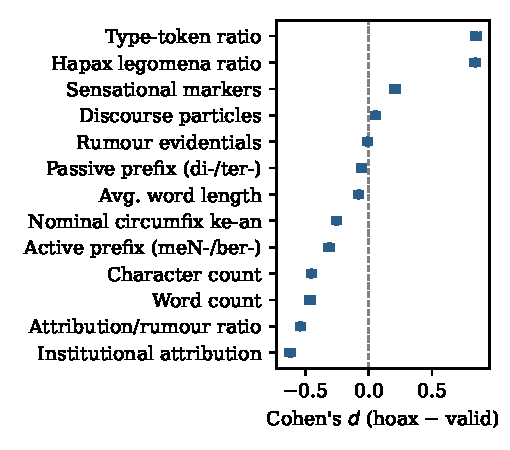
\includegraphics[width=0.62\linewidth]{figures/effect_sizes.pdf}
\caption{Effect sizes with 95\% confidence intervals. Positive values indicate higher values in hoax text.
Rumour evidentials, the feature group we expected to be most diagnostic, are indistinguishable between
classes.}
\label{fig:effects}
\end{figure}

\subsection{In-Domain Results}
\label{sec:indomain}

Tables~\ref{tab:main-original} and \ref{tab:main-normalized} give the main comparison. On the
de-duplicated \iph{} test split every model that sees tokens lands in a narrow band around
macro-F1 $0.974$--$0.978$: \menet{} reaches $0.9761{\pm}0.0054$, the text-only CNN $0.9738{\pm}0.0031$,
naive concatenation $0.9778{\pm}0.0015$ and TF-IDF with logistic regression $0.9749$. Fine-tuned
IndoBERT is the only model clearly above that band. None of the paired comparisons between \menet{} and
its ablations survives Holm correction in any condition (Table~\ref{tab:sig}): the largest absolute mean
difference is $1.4$ F1 points (\menet{} vs.\ \emph{w/o length features}, cross-dataset, normalised text,
$p_{\text{Holm}}=0.32$) and the in-domain differences are all below $0.3$ points. \textbf{On this
benchmark the gate, the symbolic stream and the individual feature groups make no measurable difference to
accuracy.} We report this as the primary empirical finding rather than searching for a condition in which
the proposed model wins.

Two secondary observations do hold consistently. First, the fused models are better calibrated than the
linear text baseline: ECE $0.012$ for the \menet{} family versus $0.053$ for TF-IDF$+$LR, a factor of four,
at equal accuracy. Second, the symbolic stream alone is far from trivial: 13 numbers with no lexical
content give macro-F1 $0.789{\pm}0.008$ (MLP) and $0.718$ (logistic regression), i.e.\ roughly
four-fifths of full performance from a 3{,}137-parameter model.

\subsection{Evidence of Shortcuts}
\label{sec:shortcuts}

The narrow band above is easier to interpret next to two controls. A logistic regression on \emph{two
features}, word count and character count, reaches macro-F1 $0.638$ in-domain, and format normalisation
changes almost nothing anywhere: the CNN moves from $0.9738$ to $0.9738$ and \menet{} from $0.9761$ to
$0.9763$, so casing and punctuation are not the carrier of the signal, but length and topic-specific
vocabulary are available in both views. In other words, a substantial part of what any model learns here
is a property of how the corpus was assembled (short social-media hoax posts versus long wire-service
articles), not of deceptive language as such \citep{gururangan2018annotation,geirhos2020shortcut}.

Cross-dataset transfer confirms this. On Rahutomo-600, where both classes are full-length articles
labelled by referees rather than scraped from different pipelines, every system collapses towards chance:
\menet{} $0.521{\pm}0.015$, the CNN $0.520{\pm}0.012$, naive concatenation $0.532{\pm}0.011$,
TF-IDF$+$LR $0.548$, and IndoBERT, the strongest in-domain model by a wide margin, $0.557$. The ranking
in-domain therefore carries essentially no information about transfer, and a 124M-parameter transformer
buys nothing out of domain despite a $+1.7$-point in-domain advantage. Calibration degrades in parallel:
ECE rises from $0.012$ to $0.288$ for \menet{} and from $0.007$ to $0.401$ for IndoBERT, so the models are
not merely wrong out of domain, they are confidently wrong. The symbolic-only models are the exception
worth noting: at chance-level accuracy they remain comparatively calibrated (ECE $0.15$--$0.19$).

\begin{figure}[t]
\centering
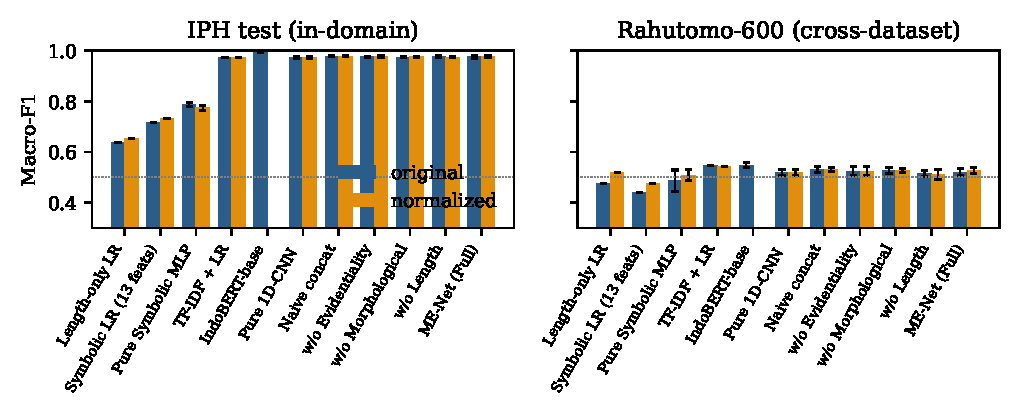
\includegraphics[width=\linewidth]{figures/indomain_vs_crossdataset.pdf}
\caption{Macro-F1 in-domain (left) and cross-dataset (right) for both input settings; bars are means over
seeds with standard-deviation whiskers. The dotted line marks chance-level macro-F1. In-domain separation
between token-based models is within noise, and no model transfers.}
\label{fig:indomain-vs-ood}
\end{figure}

\subsection{What the Gate Learns}
\label{sec:gateresults}

Because $\bar g$ of Eq.~\eqref{eq:gbar} is part of the forward pass, we can ask what the trained model
relies on without post-hoc attribution. Averaged over 10 seeds, the mean gate is
$\bar g=0.326{\pm}0.020$ for documents labelled hoax and $0.389{\pm}0.045$ for valid ones on the
in-domain test set: both classes sit below $0.5$, i.e.\ the fused representation is drawn more from the
symbolic stream than from the contextual one, and the shift between classes is small but systematic
across seeds (Figure~\ref{fig:gate}). On Rahutomo-600 the class difference vanishes
($0.361{\pm}0.034$ vs.\ $0.359{\pm}0.033$), matching the accuracy collapse: out of domain the gate no
longer discriminates, which is exactly the diagnostic signature one would want from an interpretable
component. The gate thus does something measurable and inspectable, even though it does not translate
into an accuracy gain here.

\begin{figure}[t]
\centering
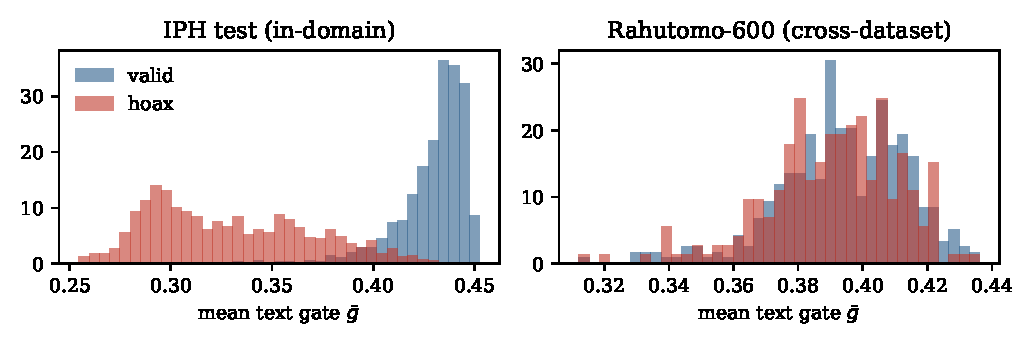
\includegraphics[width=\linewidth]{figures/gate_distribution.pdf}
\caption{Distribution of the mean gate $\bar g$ per document (first seed). In-domain (left) the two classes
separate slightly; cross-dataset (right) they coincide.}
\label{fig:gate}
\end{figure}

\subsection{Cost}
\label{sec:cost}

\menet{} has 4.03M parameters and trains in $3.6$s per run on one GPU, versus $2.2$s for the text-only CNN
and $374$s for IndoBERT (124M parameters), i.e.\ the symbolic stream and gate cost about 60\% more training
time than a bare CNN and two orders of magnitude less than fine-tuning a transformer, while the profiler
itself is a single linear pass over the text.

\begin{table}[t]
\centering\small
\caption{Main results on original text. Mean $\pm$ standard deviation over $n$ seeds (deterministic models
have $n{=}1$). Best per column in bold; ECE lower is better.}
\label{tab:main-original}
\begin{adjustbox}{max width=\linewidth}
\begin{tabular}{lccccccc}
\toprule
& & \multicolumn{3}{c}{\iph{} test (in-domain)} & \multicolumn{3}{c}{Rahutomo-600 (cross-dataset)} \\
\cmidrule(lr){3-5}\cmidrule(lr){6-8}
Model & $n$ & Macro-F1 & ROC-AUC & ECE & Macro-F1 & ROC-AUC & ECE \\
\midrule
Length-only LR & 1 & 0.638 & 0.757 & 0.099 & 0.477 & 0.447 & \textbf{0.113} \\
Symbolic LR (13 feats) & 1 & 0.718 & 0.796 & 0.053 & 0.439 & 0.488 & 0.146 \\
Pure Symbolic MLP & 10 & 0.788\,{\scriptsize$\pm$0.008} & 0.859\,{\scriptsize$\pm$0.005} & 0.066\,{\scriptsize$\pm$0.010} & 0.487\,{\scriptsize$\pm$0.042} & 0.544\,{\scriptsize$\pm$0.011} & 0.185\,{\scriptsize$\pm$0.011} \\
\midrule
TF-IDF + LR & 1 & 0.975 & 0.998 & 0.053 & 0.548 & 0.543 & 0.174 \\
IndoBERT-base (fine-tuned) & 2 & \textbf{0.992\,{\scriptsize$\pm$0.000}} & \textbf{1.000\,{\scriptsize$\pm$0.000}} & \textbf{0.008\,{\scriptsize$\pm$0.000}} & \textbf{0.549\,{\scriptsize$\pm$0.012}} & \textbf{0.595\,{\scriptsize$\pm$0.001}} & 0.404\,{\scriptsize$\pm$0.005} \\
\midrule
Pure 1D-CNN (w/o Symbolic) & 10 & 0.974\,{\scriptsize$\pm$0.003} & 0.997\,{\scriptsize$\pm$0.000} & 0.013\,{\scriptsize$\pm$0.002} & 0.520\,{\scriptsize$\pm$0.012} & 0.546\,{\scriptsize$\pm$0.009} & 0.320\,{\scriptsize$\pm$0.021} \\
Naive Concatenation (w/o Gate) & 10 & 0.978\,{\scriptsize$\pm$0.002} & 0.998\,{\scriptsize$\pm$0.000} & 0.011\,{\scriptsize$\pm$0.002} & 0.532\,{\scriptsize$\pm$0.011} & 0.558\,{\scriptsize$\pm$0.009} & 0.288\,{\scriptsize$\pm$0.013} \\
ME-Net w/o Evidentiality Priors & 10 & 0.975\,{\scriptsize$\pm$0.002} & 0.997\,{\scriptsize$\pm$0.000} & 0.013\,{\scriptsize$\pm$0.003} & 0.525\,{\scriptsize$\pm$0.018} & 0.547\,{\scriptsize$\pm$0.011} & 0.303\,{\scriptsize$\pm$0.024} \\
ME-Net w/o Morphological Priors & 10 & 0.975\,{\scriptsize$\pm$0.003} & 0.997\,{\scriptsize$\pm$0.000} & 0.014\,{\scriptsize$\pm$0.003} & 0.527\,{\scriptsize$\pm$0.012} & 0.551\,{\scriptsize$\pm$0.008} & 0.294\,{\scriptsize$\pm$0.024} \\
ME-Net w/o Length Features & 10 & 0.977\,{\scriptsize$\pm$0.004} & 0.997\,{\scriptsize$\pm$0.000} & 0.014\,{\scriptsize$\pm$0.002} & 0.516\,{\scriptsize$\pm$0.011} & 0.544\,{\scriptsize$\pm$0.008} & 0.309\,{\scriptsize$\pm$0.012} \\
\midrule
ME-Net (Full) & 10 & 0.976\,{\scriptsize$\pm$0.005} & 0.997\,{\scriptsize$\pm$0.000} & 0.012\,{\scriptsize$\pm$0.003} & 0.521\,{\scriptsize$\pm$0.015} & 0.557\,{\scriptsize$\pm$0.007} & 0.288\,{\scriptsize$\pm$0.024} \\
\bottomrule
\end{tabular}%

\end{adjustbox}
\end{table}

\begin{table}[t]
\centering\small
\caption{Main results on format-normalised text (lower-cased, punctuation removed).}
\label{tab:main-normalized}
\begin{adjustbox}{max width=\linewidth}
\begin{tabular}{lccccccc}
\toprule
& & \multicolumn{3}{c}{\iph{} test (in-domain)} & \multicolumn{3}{c}{Rahutomo-600 (cross-dataset)} \\
\cmidrule(lr){3-5}\cmidrule(lr){6-8}
Model & $n$ & Macro-F1 & ROC-AUC & ECE & Macro-F1 & ROC-AUC & ECE \\
\midrule
Length-only LR & 1 & 0.654 & 0.783 & 0.117 & 0.521 & 0.484 & \textbf{0.104} \\
Symbolic LR (13 feats) & 1 & 0.733 & 0.799 & 0.057 & 0.475 & 0.529 & 0.115 \\
Pure Symbolic MLP & 10 & 0.775\,{\scriptsize$\pm$0.011} & 0.846\,{\scriptsize$\pm$0.005} & 0.074\,{\scriptsize$\pm$0.014} & 0.509\,{\scriptsize$\pm$0.022} & 0.554\,{\scriptsize$\pm$0.004} & 0.148\,{\scriptsize$\pm$0.011} \\
\midrule
TF-IDF + LR & 1 & 0.975 & \textbf{0.998} & 0.053 & \textbf{0.544} & 0.544 & 0.164 \\
\midrule
Pure 1D-CNN (w/o Symbolic) & 10 & 0.974\,{\scriptsize$\pm$0.003} & 0.997\,{\scriptsize$\pm$0.000} & 0.013\,{\scriptsize$\pm$0.002} & 0.520\,{\scriptsize$\pm$0.012} & 0.546\,{\scriptsize$\pm$0.009} & 0.320\,{\scriptsize$\pm$0.021} \\
Naive Concatenation (w/o Gate) & 10 & \textbf{0.978\,{\scriptsize$\pm$0.001}} & 0.998\,{\scriptsize$\pm$0.000} & \textbf{0.012\,{\scriptsize$\pm$0.002}} & 0.530\,{\scriptsize$\pm$0.008} & 0.557\,{\scriptsize$\pm$0.008} & 0.298\,{\scriptsize$\pm$0.013} \\
ME-Net w/o Evidentiality Priors & 10 & 0.976\,{\scriptsize$\pm$0.003} & 0.997\,{\scriptsize$\pm$0.000} & 0.014\,{\scriptsize$\pm$0.002} & 0.525\,{\scriptsize$\pm$0.018} & 0.547\,{\scriptsize$\pm$0.010} & 0.311\,{\scriptsize$\pm$0.021} \\
ME-Net w/o Morphological Priors & 10 & 0.975\,{\scriptsize$\pm$0.003} & 0.997\,{\scriptsize$\pm$0.000} & 0.012\,{\scriptsize$\pm$0.003} & 0.527\,{\scriptsize$\pm$0.007} & 0.556\,{\scriptsize$\pm$0.007} & 0.299\,{\scriptsize$\pm$0.027} \\
ME-Net w/o Length Features & 10 & 0.975\,{\scriptsize$\pm$0.004} & 0.997\,{\scriptsize$\pm$0.000} & 0.012\,{\scriptsize$\pm$0.003} & 0.512\,{\scriptsize$\pm$0.019} & 0.551\,{\scriptsize$\pm$0.010} & 0.322\,{\scriptsize$\pm$0.030} \\
\midrule
ME-Net (Full) & 10 & 0.976\,{\scriptsize$\pm$0.004} & 0.997\,{\scriptsize$\pm$0.000} & 0.012\,{\scriptsize$\pm$0.002} & 0.527\,{\scriptsize$\pm$0.011} & \textbf{0.561\,{\scriptsize$\pm$0.006}} & 0.296\,{\scriptsize$\pm$0.028} \\
\bottomrule
\end{tabular}%

\end{adjustbox}
\end{table}

\begin{table}[t]
\centering\small
\caption{Paired differences in macro-F1 (percentage points) between \menet{} and each ablation over the
same 10 seeds, with the number of seeds on which \menet{} is better. Positive means \menet{} is better.
$^{*}$ marks $p_{\text{Holm}}<0.05$ (two-sided Wilcoxon signed-rank, corrected over the five comparisons
per condition); no comparison reaches it.}
\label{tab:sig}
\begin{adjustbox}{max width=\linewidth}
\begin{tabular}{lcccc}
\toprule
& \multicolumn{2}{c}{Original text} & \multicolumn{2}{c}{Normalised text} \\
\cmidrule(lr){2-3}\cmidrule(lr){4-5}
Comparison (\menet{} $-$ variant) & in-domain & cross-dataset & in-domain & cross-dataset \\
\midrule
Pure 1D-CNN (w/o Symbolic) & +0.23 (6/10) & +0.16 (5/10) & +0.25 (6/10) & +0.71 (6/10) \\
Naive Concatenation (w/o Gate) & -0.18 (4/10) & -1.11 (2/10) & -0.14 (3/10) & -0.32 (4/10) \\
ME-Net w/o Evidentiality Priors & +0.07 (5/10) & -0.39 (3/10) & -0.01 (4/10) & +0.17 (5/10) \\
ME-Net w/o Morphological Priors & +0.13 (4/10) & -0.59 (4/10) & +0.09 (7/10) & -0.08 (5/10) \\
ME-Net w/o Length Features & -0.09 (5/10) & +0.51 (5/10) & +0.12 (5/10) & +1.41 (7/10) \\
\bottomrule
\end{tabular}%

\end{adjustbox}
\end{table}

\section{Discussion}
\label{sec:discussion}

\paragraph{A well-specified architecture can still fail to help.}
\menet{} is strictly more expressive than the concatenation baseline (Proposition~\ref{prop:concat}), adds
linguistically motivated evidence that is individually significant (\S\ref{sec:featresults}), and costs
2.4\% extra parameters. None of that translates into accuracy on \iph{}. The most plausible explanation is
not that the architecture is wrong but that the benchmark leaves nothing for it to do: a bag of word
$n$-grams already reaches $0.975$, two length features alone reach $0.638$, and the residual error is
small enough that a 13-dimensional prior cannot move it. Architectural claims should therefore be made on
benchmarks with headroom; we would rather report this plainly than present a tuned configuration in which
the difference happens to reach significance.

\paragraph{The corpus, not the model, is the bottleneck.}
The combination of in-domain saturation and cross-dataset collapse (\S\ref{sec:shortcuts}) is the
signature of provenance-correlated construction: hoaxes and valid news enter the corpus through different
pipelines, so the label is partly predictable from document form. Our de-duplication step removed 153
validation/test documents that occurred verbatim in training, which is a second, more mundane instance of
the same problem. Format normalisation did \emph{not} change results, which rules out casing and
punctuation specifically but leaves length and topical vocabulary. For Indonesian misinformation research
the practical implication is that new resources should sample both classes from comparable venues and
lengths, and that reported numbers should always be accompanied by an out-of-corpus test; on this point
our results agree with the wider shortcut-learning literature
\citep{gururangan2018annotation,mccoy2019right,geirhos2020shortcut}.

\paragraph{Which linguistic hypotheses survived.}
The evidential hypothesis survived only in its negative half. Rumour markers are not more frequent in
hoaxes ($d=-0.009$), but institutional attribution is markedly \emph{rarer} ($d=-0.62$), and the
attribution/rumour ratio inherits that separation. This is a claim about what deceptive Indonesian text
lacks rather than what it contains, and it is robust to length normalisation by construction
(Proposition~\ref{prop:scale}). The morphological hypothesis fared less well: active-prefix and
\emph{ke-an} rates differ in the predicted direction with small effects, and passive voice, the feature we
expected to mark agentless insinuation, does not separate the classes at all.

\paragraph{What the gate is good for.}
The gate provides a cheap, built-in diagnostic: $\bar g$ separates the classes in-domain and stops doing so
exactly where the model stops transferring (\S\ref{sec:gateresults}). Used this way, a gated dual-stream
model is a probe for whether a deployment distribution still resembles the training distribution, which is
independent of whether gating improves accuracy. That said, $\bar g$ is a summary statistic of a
$128$-dimensional gate; it tells us how much a prediction leans on each view, not which feature drove it.

\paragraph{Limitations.}
(i) We train on a single corpus and test transfer on a single 600-document corpus from a different
period and topic mix; the cross-dataset numbers show that transfer fails but cannot say why.
(ii) We deliberately ran a fixed budget (5 epochs, no early stopping, no hyperparameter search) for every
neural model, which keeps the comparison clean but leaves open whether a tuned \menet{} would separate from
a tuned CNN; with all differences well inside one standard deviation, we consider a large tuned gap
unlikely. (iii) The contextual stream is a CNN, so our ablations speak about gating symbolic features into
a convolutional encoder, not into a pre-trained transformer, where the symbolic prior may be more or less
redundant. (iv) The symbolic profile is lexicon-driven, so its recall depends on 48 hand-listed markers and
a 29{,}931-entry root lexicon; morphologically productive coinages and code-mixed text are only partly
covered. (v) IndoBERT was fine-tuned with fewer seeds than the small models, so its in-domain advantage is
established less precisely, though its margin is far larger than the seed variance we observe elsewhere.

\paragraph{Future work.}
The architecture deserves a test where the label is not predictable from provenance: claim-level corpora,
same-source pairs (a hoax and its fact-check rewritten to the same length), or adversarially filtered
splits. Replacing the contextual stream with IndoBERT while keeping the gate would measure whether the
symbolic prior is redundant given pre-training. Finally, both propositions in \S\ref{sec:fusion} are
language-independent, so the same construction can be instantiated for other morphologically rich
languages by swapping $\bm{\Phi}$.


\bibliographystyle{plainnat}
\bibliography{references}

\appendix
\section{Derivation of the Gate Jacobians}
\label{app:jacobian}

We derive Proposition~\ref{prop:grad}. Write $\mathbf{q}=\mathbf{W}_g[\mathbf{z}_t;\mathbf{z}_\ell]+\mathbf{b}_g$ with
$\mathbf{W}_g=[\mathbf{W}_g^{[t]}\;\;\mathbf{W}_g^{[\ell]}]$, so $\mathbf{g}=\sigma(\mathbf{q})$ and
$\partial\mathbf{g}/\partial\mathbf{q}=\operatorname{diag}(\mathbf{g}\odot(\mathbf{1}-\mathbf{g}))=:\operatorname{diag}(\bm{\delta})$.
The pre-norm fused state is
\begin{equation}
\mathbf{s}=\mathbf{A}(\mathbf{g}\odot\mathbf{z}_t)+\mathbf{B}\big((\mathbf{1}-\mathbf{g})\odot\mathbf{z}_\ell\big)+\mathbf{b}_u .
\end{equation}
Differentiating with respect to $\mathbf{z}_t$ and using $\partial(\mathbf{g}\odot\mathbf{z}_t)/\partial\mathbf{z}_t
=\operatorname{diag}(\mathbf{g})+\operatorname{diag}(\mathbf{z}_t)\,\partial\mathbf{g}/\partial\mathbf{z}_t$ with
$\partial\mathbf{g}/\partial\mathbf{z}_t=\operatorname{diag}(\bm{\delta})\mathbf{W}_g^{[t]}$,
\begin{align}
\frac{\partial\mathbf{s}}{\partial\mathbf{z}_t}
&=\mathbf{A}\operatorname{diag}(\mathbf{g})
+\mathbf{A}\operatorname{diag}(\mathbf{z}_t)\operatorname{diag}(\bm{\delta})\mathbf{W}_g^{[t]}
-\mathbf{B}\operatorname{diag}(\mathbf{z}_\ell)\operatorname{diag}(\bm{\delta})\mathbf{W}_g^{[t]}\\
&=\mathbf{A}\operatorname{diag}(\mathbf{g})
+\big(\mathbf{A}\operatorname{diag}(\mathbf{z}_t)-\mathbf{B}\operatorname{diag}(\mathbf{z}_\ell)\big)\operatorname{diag}(\bm{\delta})\mathbf{W}_g^{[t]},
\end{align}
the minus sign coming from $\partial(\mathbf{1}-\mathbf{g})/\partial\mathbf{z}_t=-\partial\mathbf{g}/\partial\mathbf{z}_t$.
The expression for $\partial\mathbf{s}/\partial\mathbf{z}_\ell$ follows by symmetry with
$\mathbf{B}\operatorname{diag}(\mathbf{1}-\mathbf{g})$ as the leading term and $\mathbf{W}_g^{[\ell]}$ in the feedback term.

Two consequences are worth noting. First, since $\bm{\delta}=\mathbf{g}\odot(\mathbf{1}-\mathbf{g})\le\frac14$
element-wise, the feedback terms are bounded relative to the leading terms whenever
$\lVert\mathbf{W}_g\rVert$ is moderate, so the gate behaves like a smooth interpolation rather than a hard
switch early in training. Second, a saturated coordinate ($g_j\!\to\!0$ or $1$) has
$\delta_j\!\to\!0$, so it stops updating the gate itself: saturation is self-reinforcing, which is why we
report the empirical distribution of $\bar g$ rather than assuming the gate stays in its linear regime.

\section{Feature Extraction Complexity}
\label{app:complexity}

Algorithm~\ref{alg:profile} extracts $\bm{\Phi}$ in a single pass. With memoised per-token decisions, the
amortised cost per token is $O(1)$ hash lookups: at most $|\mathrm{Pre}_{\text{pas}}|+|\mathrm{Pre}_{\text{act}}|=11$
prefix tests, each with at most two allomorph restorations, and at most $|\mathcal{C}|=4$ clitic tests.
Regular-expression matching over the three marker lexicons is linear in document length. Total cost is
therefore $\Theta(N)$ per document with a small constant, independent of the neural configuration.

\begin{algorithm}[h]
\caption{Morpho-evidential profile $\bm{\Phi}$}
\label{alg:profile}
\begin{algorithmic}[1]
\Require document text; root lexicon $\mathcal{L}$; exception sets; marker lexicons
\State $w\gets$ lower-cased word tokens; $N\gets\max(|w|,1)$
\State $c_{\text{pas}},c_{\text{act}},c_{\text{ke}},c_{\text{prt}}\gets0$
\For{each token $t\in w$}
  \If{$\pi_{\text{pas}}(t)$} $c_{\text{pas}}{+}{+}$
  \ElsIf{$\pi_{\text{act}}(t)$} $c_{\text{act}}{+}{+}$
  \ElsIf{$\pi_{\text{ke-an}}(t)$} $c_{\text{ke}}{+}{+}$
  \EndIf
  \If{$\pi_{\text{prt}}(t)$} $c_{\text{prt}}{+}{+}$ \EndIf
\EndFor
\State $c_{\text{rum}},c_{\text{ins}},c_{\text{sen}}\gets$ regex match counts of $\mathcal{R}_{\text{rum}},\mathcal{R}_{\text{ins}},\mathcal{R}_{\text{sen}}$
\State convert all counts to rates by Eq.~\eqref{eq:rate}; compute $\Psi$ by Eq.~\eqref{eq:ratio}
\State \Return $[\,N,\;|\text{text}|_{\text{ch}},\;\bar\lambda,\;\mathrm{TTR},\;\mathrm{HPX},\;r_{\text{pas}},r_{\text{act}},r_{\text{ke-an}},r_{\text{prt}},r_{\text{rum}},r_{\text{ins}},r_{\text{sen}},\Psi\,]$
\end{algorithmic}
\end{algorithm}

\section{Hyperparameters}
\label{app:hyper}

\begin{table}[h]
\centering\small
\caption{Training configuration shared by all neural models.}
\begin{tabular}{ll}
\toprule
Setting & Value \\
\midrule
Vocabulary / min.\ token frequency & 30{,}000 / 2 \\
Sequence length $L$ & 256 \\
Embedding / filters / fusion width & 128 / 128 / 128 \\
Convolution width $k$ & 5 \\
Symbolic encoder width $d_\ell$ & 64 \\
Dropout (encoder / fusion) & 0.3 / 0.2 \\
Optimiser & AdamW, $\eta=10^{-3}$, $\lambda=10^{-4}$ \\
Batch size / epochs & 64 / 5 \\
Seeds & 13, 21, 42, 87, 100, 123, 256, 512, 777, 1024 \\
\bottomrule
\end{tabular}
\end{table}


\end{document}
